\RequirePackage{plautopatch}
\documentclass[english, dvipdfmx, a4paper]{jsarticle}
\usepackage[utf8]{inputenc}
\usepackage[top=10truemm, bottom=20truemm, left=15truemm, right=15truemm]{geometry} % mergin
\renewcommand{\headfont}{\bfseries}

% graphics
\usepackage{graphicx}
\usepackage{here}

% link

\usepackage{url}
\usepackage[dvipdfmx, linktocpage]{hyperref} 
\usepackage{xcolor}
\usepackage{pxjahyper}
\hypersetup{
	colorlinks=true,
	citecolor=blue,
	linkcolor=teal,
	urlcolor=orange,
}

% math
\usepackage{tikz}
\usepackage[all]{xy}
\usepackage{amsmath, amssymb} 
\usepackage{physics}
\usepackage{mathrsfs}
\usepackage{mathtools}

% theoremstyle
\usepackage{amsthm}
\newtheoremstyle{break}
{\topsep}{\topsep}%
{}{}%
{\bfseries}{}%
{\newline}{}%
\theoremstyle{break}
\newtheorem{thm}{Theorem}[section]
\newtheorem{defn}[thm]{Definition}
\newtheorem{eg}[thm]{Example}
\newtheorem{cl}[thm]{Claim}
\newtheorem{cor}[thm]{Corollary}
\newtheorem{fact}[thm]{Fact}
\newtheorem{rem}[thm]{Remark}
\newtheorem{prob}{Problem}[section]

\makeatletter
\newenvironment{pr}[1][\proofnam]{\par
\topsep6\p@\@plus6\p@ \trivlist
\item[\hskip\labelsep{\itshape #1}\@addpunct{\bfseries}]\ignorespaces
}{%
\endtrivlist
}
\newcommand{\proofnam}{\underline{Proof.}}
\makeatother


% my command

\newcommand{\R}{\mathbb{R}}
\newcommand{\C}{\mathbb{C}}
\newcommand{\Z}{\mathbb{Z}}

\newcommand{\eq}[1]{Eq. \eqref{#1}}
\newcommand{\theorem}[1]{Thm. \ref{#1}}
\newcommand{\definition}[1]{Def. \ref{#1}}
\newcommand{\proposition}[1]{Prop. \ref{#1}}
\newcommand{\example}[1]{e.g.\ref{#1}}
\newcommand{\claim}[1]{Cl. \ref{#1}}
\newcommand{\corolary}[1]{Cor. \ref{#1}}
\newcommand{\remark}[1]{Rem. \ref{#1}}
\newcommand{\problem}[1]{Prob. \ref{#1}}
\newcommand{\slashed}[1]{#1\!\!\!/}
\renewcommand{\O}{\mathcal{O}}


% number

%\makeatletter
%\@addtoreset{equation}{section}
%\makeatother
%\numberwithin{equation}{section}
%\renewcommand{\thefootnote}{\roman{footnote}.}
%\renewcommand{\appendixname}{Appendix }

\title{ブラックホールの情報喪失問題}
\author{Yuji Tachikawa}
\date{\today}

\begin{document}
	\maketitle
	\begin{abstract}
			一般相対論,熱統計力学,量子力学の三つのそれぞれには自己矛盾はないが,三つを組み合わせると矛盾しているように思われる.この例がブラックホールの情報喪失問題である.このような状況は現在の理論物理では珍しい.

			一般相対論によると,とても重くて小さいものは光も吸い込むブラックホールとよばれる天体になる\cite{Schwarzschild:1916uq}.そのブラックホールを量子力学的に扱うと熱的な放射があることがわかる\cite{Hawking:1974rv}.
			ブラックホールは熱的な放射によりエネルギーを失い,やがて消滅すると思われている.

			さて,ブラックホールは古典一般相対論では何を圧縮してつくっても全質量$M $にしかよらない.Hawking輻射も$M $にしかよらない.蒸発すると,もともと何でできていたかという情報が失われてしまう.ところが,量子力学では原理的に情報は失われないはずである.これがブラックホールの情報喪失問題である.

			この問題は現時点でも解決されておらず,本稿では一体どういう問題なのか理解することを目標にする.
	\end{abstract}
	\tableofcontents
	\section{特殊相対論}
特殊相対論は平らな空間の幾何である.

\begin{enumerate}
		\item 初等幾何的アプローチ\label{enu:intro_first}
		\item 座標幾何的アプローチ\label{enu:intro_second}
\end{enumerate}
がある.よくある教科書では\ref{enu:intro_first}が多い気がする.
今回は\ref{enu:intro_second}でやる.

原点$(0, 0) $と時空点$(t, x) $について,
$t^2 -x^2 > 0 $ならば,$\tau^2\coloneqq t^2 - x^2 $として$\tau $を固有時間,$t^2 - x-2 < 0 $ならば$x_0^2\coloneqq x^2 - t^2 $として$x_0 $を固有長さという.

Lorentz変換とは$(t)^2 - x^2 $を保つ線形な座標変換のことである.
\begin{table}[htbp]
		\centering
		\label{tab:Lorentz-rotation}
		\caption{平面幾何での回転とローレンツ変換}
		\begin{tabular}{c|cc}\hline
				 & 平面幾何 & 特殊相対論\\\hline
				大切なもの & $x^2 + y^2 $ & $t^2 - x^2 $\\
				それを保つ変換 & 回転 & Lorentz変換\\\hline
		\end{tabular}
\end{table}

二点$(t, x) $, $(t', x') $に対し,$t^2 -x^2 = (t')^2 - (x')^2 $を要求すると,$(t-x)(t+x) = (t'-x')(t'+x') $であり,$\eta\in\R $が存在して
\begin{align}
		t' + x' &= e^{\eta}(t + x),\\
		t' - x' &= e^{-\eta}(t-x)
\end{align}とかける.

\begin{align}
		\begin{pmatrix}
				t'\\
				x'
		\end{pmatrix}
		&=
		\begin{pmatrix}
				(e^\eta + e^{-\eta})/2 & (e^{\eta} - e^{-\eta})/2\\
				(e^{\eta}-e^{-\eta})/2 & (e^{\eta}+e^{-\eta})/2
		\end{pmatrix}
		\begin{pmatrix}
				t\\
				x
		\end{pmatrix}
		\\
		&= \begin{pmatrix}
				\cosh\eta & \sinh\eta\\
				\sinh\eta & \cosh\eta
		\end{pmatrix}
		\begin{pmatrix}
				t\\
				x
		\end{pmatrix}
\end{align}
となる.パラメータ$\eta $をLorentz変換のrapidityという.

Lorentz変換は
\begin{align}
		\cosh^2\eta - \sinh^2\eta &= 1,\\
		\cosh(\eta + \xi) &= \cosh\eta \cosh\xi + \sinh\eta\sinh\xi,\\
		\sinh(\eta + \xi) &= \sinh\eta \cosh\xi + \cosh\eta\sinh\xi
\end{align}
を満たす.

回転も同様で角$\theta $の回転とは
\begin{equation}
		\begin{pmatrix}
				x'\\
				y'
		\end{pmatrix}
		= 
		\begin{pmatrix}
				\cos\theta & -\sin\theta\\
				\sin\theta & \cos \theta
		\end{pmatrix}
		\begin{pmatrix}
				x\\
				y
		\end{pmatrix}
\end{equation}
である.

まとめると,表\ref{tab:trig_hypo}のようになる.
\begin{table}[htbp]
		\centering
		\caption{回転とLorentz変換の比較.}
		\begin{tabular}{cc}\hline
				回転 & Lorentz変換\\\hline
				\begin{minipage}{0.45\textwidth}
					\centering
					\scalebox{0.5}{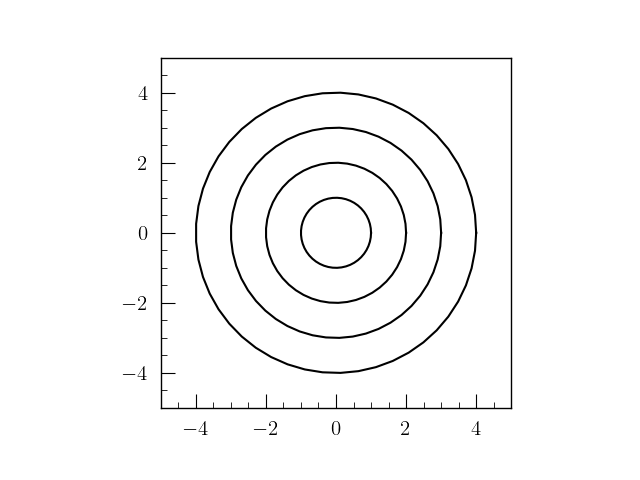
\includegraphics{./img/rotation.png}}
					\caption{$x^2 + y^2$一定.}
			    \end{minipage} &
			    \begin{minipage}{0.45\textwidth}
			    	\centering
					\scalebox{0.5}{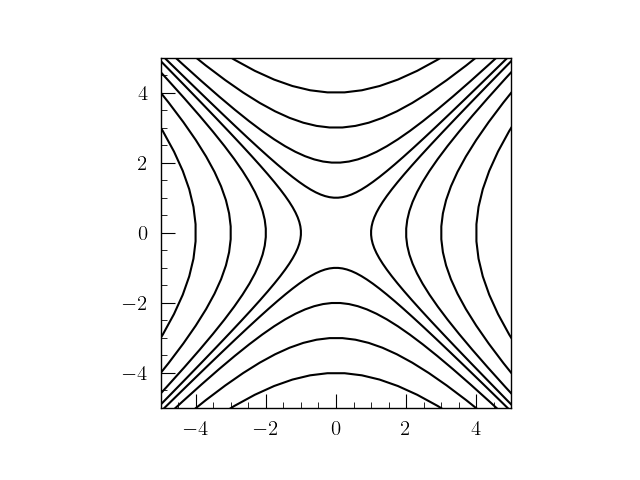
\includegraphics{./img/boost.png}}
					\caption{$t^2 - x^2$一定.}
			    \end{minipage}\\
					 & \\\hline
				$x' + y' = e^{i\theta}(x + y) $ & $t' + x' = e^{\eta}(t+x) $\\
				$x' - y' = e^{-i\theta}(x-y) $ & $t'-x' = e^{-\eta}(t-x)$\\\hline
				三角関数$\sin $, $\cos $ & 双曲線関数$\sinh $, $\cosh $\\\hline

		\end{tabular}
		\label{tab:trig_hypo}
\end{table}

		特殊相対論には(数学的には)Euclid幾何以上に不思議なことはなにもない.\footnote{$i$を使わない分マシとも言える.}

	\section{一般相対論}

Newtonの重力理論は特殊相対論とは相容れない.平らな時空の幾何である特殊相対論をまがった時空に拡張した一般相対論というものになる.

そのまえに「力」とは?Newtonの運動方程式$F = ma $の$F $だが,摩擦力などいろいろあるが,突き詰めれば重力,電磁気力,弱い力\footnote{$\beta $崩壊を起こす.},強い力\footnote{quarkを陽子,中性子などにまとめる力.}の四つである\footnote{強い力,弱い力は常に量子的に考える.}.

力の統一については
\begin{align}
		\xymatrix{
& \text{重力} & \\
				\text{電弱力} &\ar[l]\text{電磁気力} & \ar[l] \text{電気力}\\
				& \ar[ul]^{\text{Glashow--Weinberg--Salam}}\text{弱い力} & \ar[ul]_{\text{Maxwell}}\text{磁気力}\\
				& \text{強い力} & 
		}\notag
\end{align}
となっている.

各力の量子論の現状は表\ref{tab:quantum}のようである.量子重力は現状全くできていない.
\begin{table}[htbp]
		\centering
		\caption{各力の量子論.}
		\label{tab:quantum}
		\begin{tabular}{cl}\hline
				量子電磁力学 & 物理屋的には確立.\\
				量子弱い力 & 実験とよく合う.\\
				量子強い力\footnote{hoge} & 数学的にはよく定義されていない.\\\hline
				量子重力 & 
				\begin{tabular}{l}
						実験結果は全くなし.\\
						物理屋のレベルでも全然できていない.\\
						ブラックホールの情報喪失問題はその一端.
				\end{tabular}\\\hline
		\end{tabular}
\end{table}

	\section{最低限必要な一般相対論}
一般相対論の方程式のためには曲がった空間の幾何を学ばねばならない.
大変だが,大部分は機械的にできる.

例えば,平面だと直線が最短ルートである.球面は一様に曲がっており.大円が最短である.もっと一般的な曲面では二点間上の最短経路を測地線(geodesic)という.もっと抽象的に埋め込みなしにそれ自身曲がっているものを考えてもよい.
hoge

	\bibliography{komaba}
	\bibliographystyle{ytamsalpha}
	%\bibliographystyle{ytamsbeta}
\end{document}

